% Options for packages loaded elsewhere
\PassOptionsToPackage{unicode}{hyperref}
\PassOptionsToPackage{hyphens}{url}
%
\documentclass[
]{article}
\usepackage{amsmath,amssymb}
\usepackage{iftex}
\ifPDFTeX
  \usepackage[T1]{fontenc}
  \usepackage[utf8]{inputenc}
  \usepackage{textcomp} % provide euro and other symbols
\else % if luatex or xetex
  \usepackage{unicode-math} % this also loads fontspec
  \defaultfontfeatures{Scale=MatchLowercase}
  \defaultfontfeatures[\rmfamily]{Ligatures=TeX,Scale=1}
\fi
\usepackage{lmodern}
\ifPDFTeX\else
  % xetex/luatex font selection
\fi
% Use upquote if available, for straight quotes in verbatim environments
\IfFileExists{upquote.sty}{\usepackage{upquote}}{}
\IfFileExists{microtype.sty}{% use microtype if available
  \usepackage[]{microtype}
  \UseMicrotypeSet[protrusion]{basicmath} % disable protrusion for tt fonts
}{}
\makeatletter
\@ifundefined{KOMAClassName}{% if non-KOMA class
  \IfFileExists{parskip.sty}{%
    \usepackage{parskip}
  }{% else
    \setlength{\parindent}{0pt}
    \setlength{\parskip}{6pt plus 2pt minus 1pt}}
}{% if KOMA class
  \KOMAoptions{parskip=half}}
\makeatother
\usepackage{xcolor}
\usepackage[margin=1in]{geometry}
\usepackage{color}
\usepackage{fancyvrb}
\newcommand{\VerbBar}{|}
\newcommand{\VERB}{\Verb[commandchars=\\\{\}]}
\DefineVerbatimEnvironment{Highlighting}{Verbatim}{commandchars=\\\{\}}
% Add ',fontsize=\small' for more characters per line
\usepackage{framed}
\definecolor{shadecolor}{RGB}{248,248,248}
\newenvironment{Shaded}{\begin{snugshade}}{\end{snugshade}}
\newcommand{\AlertTok}[1]{\textcolor[rgb]{0.94,0.16,0.16}{#1}}
\newcommand{\AnnotationTok}[1]{\textcolor[rgb]{0.56,0.35,0.01}{\textbf{\textit{#1}}}}
\newcommand{\AttributeTok}[1]{\textcolor[rgb]{0.13,0.29,0.53}{#1}}
\newcommand{\BaseNTok}[1]{\textcolor[rgb]{0.00,0.00,0.81}{#1}}
\newcommand{\BuiltInTok}[1]{#1}
\newcommand{\CharTok}[1]{\textcolor[rgb]{0.31,0.60,0.02}{#1}}
\newcommand{\CommentTok}[1]{\textcolor[rgb]{0.56,0.35,0.01}{\textit{#1}}}
\newcommand{\CommentVarTok}[1]{\textcolor[rgb]{0.56,0.35,0.01}{\textbf{\textit{#1}}}}
\newcommand{\ConstantTok}[1]{\textcolor[rgb]{0.56,0.35,0.01}{#1}}
\newcommand{\ControlFlowTok}[1]{\textcolor[rgb]{0.13,0.29,0.53}{\textbf{#1}}}
\newcommand{\DataTypeTok}[1]{\textcolor[rgb]{0.13,0.29,0.53}{#1}}
\newcommand{\DecValTok}[1]{\textcolor[rgb]{0.00,0.00,0.81}{#1}}
\newcommand{\DocumentationTok}[1]{\textcolor[rgb]{0.56,0.35,0.01}{\textbf{\textit{#1}}}}
\newcommand{\ErrorTok}[1]{\textcolor[rgb]{0.64,0.00,0.00}{\textbf{#1}}}
\newcommand{\ExtensionTok}[1]{#1}
\newcommand{\FloatTok}[1]{\textcolor[rgb]{0.00,0.00,0.81}{#1}}
\newcommand{\FunctionTok}[1]{\textcolor[rgb]{0.13,0.29,0.53}{\textbf{#1}}}
\newcommand{\ImportTok}[1]{#1}
\newcommand{\InformationTok}[1]{\textcolor[rgb]{0.56,0.35,0.01}{\textbf{\textit{#1}}}}
\newcommand{\KeywordTok}[1]{\textcolor[rgb]{0.13,0.29,0.53}{\textbf{#1}}}
\newcommand{\NormalTok}[1]{#1}
\newcommand{\OperatorTok}[1]{\textcolor[rgb]{0.81,0.36,0.00}{\textbf{#1}}}
\newcommand{\OtherTok}[1]{\textcolor[rgb]{0.56,0.35,0.01}{#1}}
\newcommand{\PreprocessorTok}[1]{\textcolor[rgb]{0.56,0.35,0.01}{\textit{#1}}}
\newcommand{\RegionMarkerTok}[1]{#1}
\newcommand{\SpecialCharTok}[1]{\textcolor[rgb]{0.81,0.36,0.00}{\textbf{#1}}}
\newcommand{\SpecialStringTok}[1]{\textcolor[rgb]{0.31,0.60,0.02}{#1}}
\newcommand{\StringTok}[1]{\textcolor[rgb]{0.31,0.60,0.02}{#1}}
\newcommand{\VariableTok}[1]{\textcolor[rgb]{0.00,0.00,0.00}{#1}}
\newcommand{\VerbatimStringTok}[1]{\textcolor[rgb]{0.31,0.60,0.02}{#1}}
\newcommand{\WarningTok}[1]{\textcolor[rgb]{0.56,0.35,0.01}{\textbf{\textit{#1}}}}
\usepackage{longtable,booktabs,array}
\usepackage{calc} % for calculating minipage widths
% Correct order of tables after \paragraph or \subparagraph
\usepackage{etoolbox}
\makeatletter
\patchcmd\longtable{\par}{\if@noskipsec\mbox{}\fi\par}{}{}
\makeatother
% Allow footnotes in longtable head/foot
\IfFileExists{footnotehyper.sty}{\usepackage{footnotehyper}}{\usepackage{footnote}}
\makesavenoteenv{longtable}
\usepackage{graphicx}
\makeatletter
\def\maxwidth{\ifdim\Gin@nat@width>\linewidth\linewidth\else\Gin@nat@width\fi}
\def\maxheight{\ifdim\Gin@nat@height>\textheight\textheight\else\Gin@nat@height\fi}
\makeatother
% Scale images if necessary, so that they will not overflow the page
% margins by default, and it is still possible to overwrite the defaults
% using explicit options in \includegraphics[width, height, ...]{}
\setkeys{Gin}{width=\maxwidth,height=\maxheight,keepaspectratio}
% Set default figure placement to htbp
\makeatletter
\def\fps@figure{htbp}
\makeatother
\setlength{\emergencystretch}{3em} % prevent overfull lines
\providecommand{\tightlist}{%
  \setlength{\itemsep}{0pt}\setlength{\parskip}{0pt}}
\setcounter{secnumdepth}{5}
\usepackage{booktabs}
\usepackage{longtable}
\usepackage{array}
\usepackage{multirow}
\usepackage{wrapfig}
\usepackage{float}
\usepackage{colortbl}
\usepackage{pdflscape}
\usepackage{tabu}
\usepackage{threeparttable}
\usepackage{threeparttablex}
\usepackage[normalem]{ulem}
\usepackage{makecell}
\usepackage{xcolor}
\usepackage{caption}
\ifLuaTeX
  \usepackage{selnolig}  % disable illegal ligatures
\fi
\IfFileExists{bookmark.sty}{\usepackage{bookmark}}{\usepackage{hyperref}}
\IfFileExists{xurl.sty}{\usepackage{xurl}}{} % add URL line breaks if available
\urlstyle{same}
\hypersetup{
  pdftitle={Week 11: Practical Example},
  pdfauthor={Monica Truelove-Hill},
  hidelinks,
  pdfcreator={LaTeX via pandoc}}

\title{Week 11: Practical Example}
\author{Monica Truelove-Hill}
\date{2023-11-14}

\begin{document}
\maketitle

{
\setcounter{tocdepth}{2}
\tableofcontents
}
\hypertarget{overview-of-the-week}{%
\section{Overview of the Week}\label{overview-of-the-week}}

This week, we'll be reviewing what we've learned in weeks 7-10 and applying it to a practical example. Specifically, we'll cover:

\begin{enumerate}
\def\labelenumi{\arabic{enumi})}
\tightlist
\item
  Multiple linear regression with categorical variables;
\item
  Dummy, effects, and manual contrast coding;
\item
  Checking model assumptions \& diagnostics;
\item
  Bootstrapping
\end{enumerate}

Our example is based on the paper \emph{\href{https://www.ucsd.ac.uk/wp-content/uploads/Benefits-of-attendance-for-students.pdf}{Class Attendance in College: A Meta-Analytic Review of the Relationship of Class Attendance With Grades and Student Characteristics}} This paper looks at the association between class attendance and a range of other variables (such as student personality, academic performance, class marks, etc.) Imagine that we've read that paper and we want to perform further investigation on the variables that contribute to attendance. Specifically, we will investigate a range of categorical variables here. We'll also use our data to try and replicate the association between attendance and marks that is found in this paper.

During this week's example, we will conduct two separate, but related, studies. In the first, we are interested in exploring possible predictors of attendance in university courses. In the second, we will investigate the association between attendance and final marks in our sample.

\hypertarget{study-1}{%
\section{Study 1}\label{study-1}}

We collected data from 397 university students across years 1-4, as well as students in MSc and PhD programs. From these students, we gathered data on class time, the use of online materials, and student's self-discipline.

\begin{longtable}{ll}
\toprule
Variable & Description \\ 
\midrule
pid & Participant ID number \\ 
Attendance & Total attendance in days \\ 
Conscientiousness & Level of conscientiousness (levels = Low; Moderate; High) \\ 
Time & Class time (levels = 9AM; 10AM; 11AM; 12PM; 1PM; 2PM; 3PM; 4PM) \\ 
OnlineAccess & Frequency of access to online course materials (levels = Rarely; Sometimes; Often) \\ 
Year & Year in university (levels = Y1; Y2; Y3; Y4; MSc; PhD) \\ 
\bottomrule
\end{longtable}

We want to use these data to investigate the following research questions:

\textbf{Research Question 1:} Can student's conscientiousness, frequency of access to online materials, and year in University predict course attendance?

\textbf{Research Question 2:} Is the time at which the class is scheduled associated with student attendance?

\hypertarget{setup}{%
\subsubsection{Setup}\label{setup}}

First, let's load the data and all necessary packages. Note that by using the \texttt{stringsAsFactors} argument in the \texttt{read.csv} function, all of our character variables are automatically imported as factors, which is very handy when you're working with a dataset with lots of factors in it.

\begin{Shaded}
\begin{Highlighting}[]
\FunctionTok{library}\NormalTok{(tidyverse)}
\FunctionTok{library}\NormalTok{(emmeans)}
\FunctionTok{library}\NormalTok{(kableExtra)}
\FunctionTok{library}\NormalTok{(car)}

\NormalTok{dat }\OtherTok{\textless{}{-}} \FunctionTok{read.csv}\NormalTok{(}\StringTok{\textquotesingle{}https://uoepsy.github.io/data/DapR2\_S1B2\_PracticalPart1.csv\textquotesingle{}}\NormalTok{, }\AttributeTok{stringsAsFactors =}\NormalTok{ T)}
\end{Highlighting}
\end{Shaded}

\hypertarget{checking-the-data}{%
\subsubsection{Checking the Data}\label{checking-the-data}}

First, we'll have a look at our data using the \texttt{summary} function:

\begin{Shaded}
\begin{Highlighting}[]
\NormalTok{dat }\SpecialCharTok{\%\textgreater{}\%}
  \FunctionTok{summary}\NormalTok{(.)}
\end{Highlighting}
\end{Shaded}

\begin{verbatim}
##       pid        Attendance    Conscientiousness      Time          
##  Min.   :  1   Min.   : 0.00   Length:397         Length:397        
##  1st Qu.:100   1st Qu.:16.00   Class :character   Class :character  
##  Median :199   Median :29.00   Mode  :character   Mode  :character  
##  Mean   :199   Mean   :28.28                                        
##  3rd Qu.:298   3rd Qu.:40.00                                        
##  Max.   :395   Max.   :60.00                                        
##  OnlineAccess           Year          
##  Length:397         Length:397        
##  Class :character   Class :character  
##  Mode  :character   Mode  :character  
##                                       
##                                       
## 
\end{verbatim}

You'll notice that we have a continuous outcome variable, \texttt{Attendance}, and discrete predictor variables, \texttt{Conscientiousness}, \texttt{Time}, \texttt{OnlineAccess} and \texttt{Year}.

We'll also have a look at how our variables are distributed, using a histogram for our continous outcome and bar plots for our factors:

\begin{Shaded}
\begin{Highlighting}[]
\FunctionTok{ggplot}\NormalTok{(dat, }\FunctionTok{aes}\NormalTok{(Attendance)) }\SpecialCharTok{+} \FunctionTok{geom\_histogram}\NormalTok{(}\AttributeTok{colour =} \StringTok{\textquotesingle{}black\textquotesingle{}}\NormalTok{, }\AttributeTok{binwidth =} \DecValTok{5}\NormalTok{)}
\end{Highlighting}
\end{Shaded}

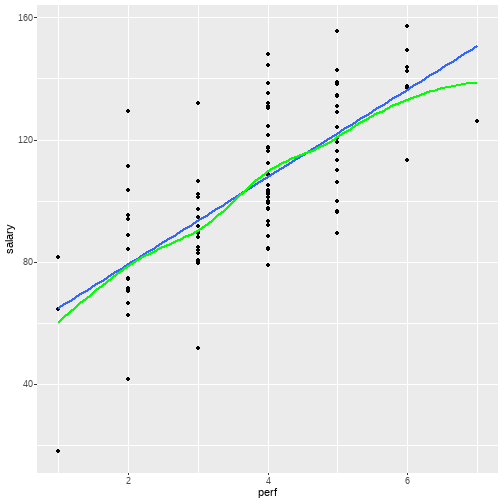
\includegraphics{dapr2_10_CategoricalAnalysisPlan_files/figure-latex/unnamed-chunk-5-1.pdf}

\begin{Shaded}
\begin{Highlighting}[]
\FunctionTok{ggplot}\NormalTok{(dat, }\FunctionTok{aes}\NormalTok{(Conscientiousness, }\AttributeTok{fill =}\NormalTok{ Conscientiousness)) }\SpecialCharTok{+} \FunctionTok{geom\_bar}\NormalTok{() }\SpecialCharTok{+}
  \FunctionTok{theme}\NormalTok{(}\AttributeTok{legend.position =} \StringTok{\textquotesingle{}none\textquotesingle{}}\NormalTok{)}
\end{Highlighting}
\end{Shaded}

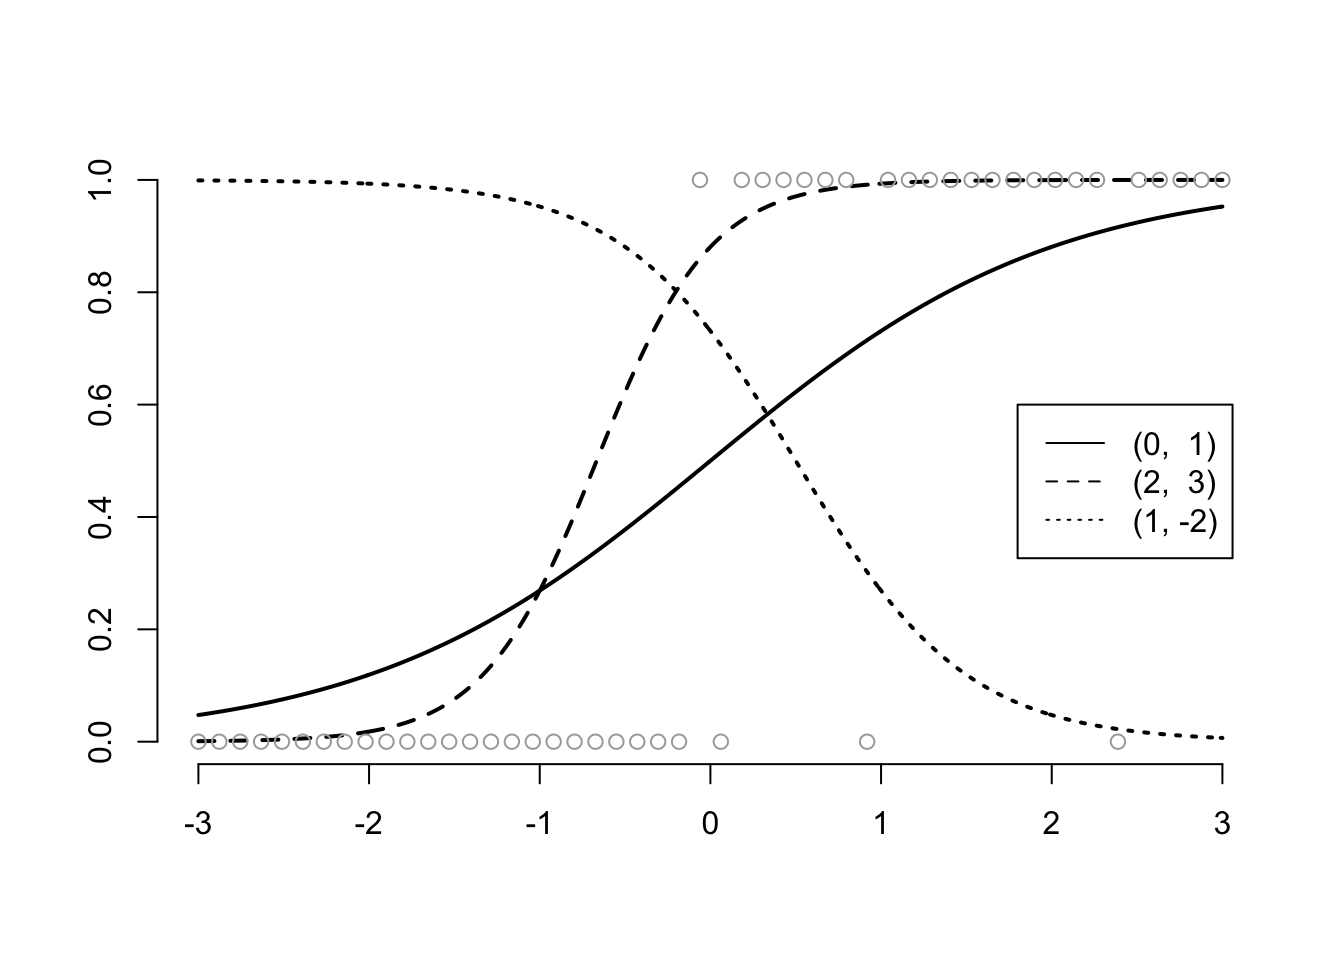
\includegraphics{dapr2_10_CategoricalAnalysisPlan_files/figure-latex/unnamed-chunk-6-1.pdf}

\begin{Shaded}
\begin{Highlighting}[]
\FunctionTok{ggplot}\NormalTok{(dat, }\FunctionTok{aes}\NormalTok{(Year, }\AttributeTok{fill =}\NormalTok{ Year)) }\SpecialCharTok{+} \FunctionTok{geom\_bar}\NormalTok{() }\SpecialCharTok{+}
  \FunctionTok{theme}\NormalTok{(}\AttributeTok{legend.position =} \StringTok{\textquotesingle{}none\textquotesingle{}}\NormalTok{)}
\end{Highlighting}
\end{Shaded}

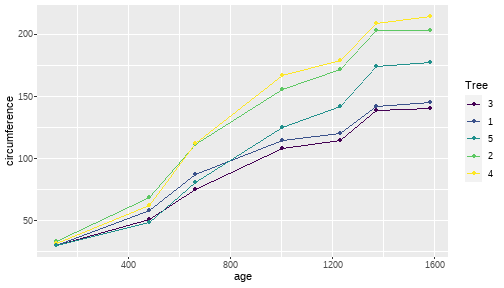
\includegraphics{dapr2_10_CategoricalAnalysisPlan_files/figure-latex/unnamed-chunk-7-1.pdf}

\begin{Shaded}
\begin{Highlighting}[]
\FunctionTok{ggplot}\NormalTok{(dat, }\FunctionTok{aes}\NormalTok{(Time, }\AttributeTok{fill =}\NormalTok{ Time)) }\SpecialCharTok{+} \FunctionTok{geom\_bar}\NormalTok{() }\SpecialCharTok{+}
  \FunctionTok{theme}\NormalTok{(}\AttributeTok{legend.position =} \StringTok{\textquotesingle{}none\textquotesingle{}}\NormalTok{)}
\end{Highlighting}
\end{Shaded}

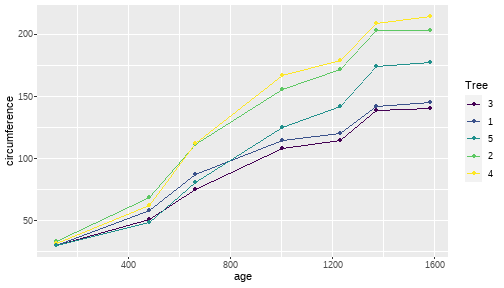
\includegraphics{dapr2_10_CategoricalAnalysisPlan_files/figure-latex/unnamed-chunk-8-1.pdf}

\hypertarget{investigating-rq-1}{%
\subsubsection{Investigating RQ 1}\label{investigating-rq-1}}

Given the first research question we've specified, \textbf{Can student's conscientiousness, frequency of access to online materials, and year in University predict course attendance?}, we'll use the following model:

\[Attendance \sim Conscientiousness + OnlineAccess + Year\]

\hypertarget{dummy-coding}{%
\paragraph{Dummy Coding}\label{dummy-coding}}

Between the 3 predictors, we have 12 levels. Before we run our model, we have to make a few decisions in terms of the coding and baseline comparisons we'll be making across predictors. We decide to use dummy coding. We'll use be using \texttt{Moderate} as the baseline level for \texttt{Conscientiousness} and \texttt{Sometimes} as the baseline level for \texttt{OnlineAccess}. We'll keep \texttt{Y1} as the baseline level for \texttt{Year}. We can use the \texttt{factor} function to order our levels accordingly:

\begin{Shaded}
\begin{Highlighting}[]
\NormalTok{dat}\SpecialCharTok{$}\NormalTok{Conscientiousness }\OtherTok{\textless{}{-}}\NormalTok{ dat}\SpecialCharTok{$}\NormalTok{Conscientiousness }\SpecialCharTok{\%\textgreater{}\%} 
  \FunctionTok{factor}\NormalTok{(., }\AttributeTok{levels =} \FunctionTok{c}\NormalTok{(}\StringTok{\textquotesingle{}Moderate\textquotesingle{}}\NormalTok{, }\StringTok{\textquotesingle{}Low\textquotesingle{}}\NormalTok{, }\StringTok{\textquotesingle{}High\textquotesingle{}}\NormalTok{))}

\FunctionTok{summary}\NormalTok{(dat}\SpecialCharTok{$}\NormalTok{Conscientiousness)}
\end{Highlighting}
\end{Shaded}

\begin{verbatim}
## Moderate      Low     High 
##      146      127      124
\end{verbatim}

\begin{Shaded}
\begin{Highlighting}[]
\NormalTok{dat}\SpecialCharTok{$}\NormalTok{OnlineAccess }\OtherTok{\textless{}{-}}\NormalTok{ dat}\SpecialCharTok{$}\NormalTok{OnlineAccess }\SpecialCharTok{\%\textgreater{}\%} 
  \FunctionTok{factor}\NormalTok{(., }\AttributeTok{levels =} \FunctionTok{c}\NormalTok{(}\StringTok{\textquotesingle{}Sometimes\textquotesingle{}}\NormalTok{, }\StringTok{\textquotesingle{}Rarely\textquotesingle{}}\NormalTok{, }\StringTok{\textquotesingle{}Often\textquotesingle{}}\NormalTok{))}

\FunctionTok{summary}\NormalTok{(dat}\SpecialCharTok{$}\NormalTok{OnlineAccess)}
\end{Highlighting}
\end{Shaded}

\begin{verbatim}
## Sometimes    Rarely     Often 
##       170       101       126
\end{verbatim}

\begin{Shaded}
\begin{Highlighting}[]
\NormalTok{dat}\SpecialCharTok{$}\NormalTok{Year }\OtherTok{\textless{}{-}}\NormalTok{ dat}\SpecialCharTok{$}\NormalTok{Year }\SpecialCharTok{\%\textgreater{}\%} 
  \FunctionTok{factor}\NormalTok{(., }\AttributeTok{levels =} \FunctionTok{c}\NormalTok{(}\StringTok{\textquotesingle{}Y1\textquotesingle{}}\NormalTok{, }\StringTok{\textquotesingle{}Y2\textquotesingle{}}\NormalTok{, }\StringTok{\textquotesingle{}Y3\textquotesingle{}}\NormalTok{, }\StringTok{\textquotesingle{}Y4\textquotesingle{}}\NormalTok{, }\StringTok{\textquotesingle{}MSc\textquotesingle{}}\NormalTok{, }\StringTok{\textquotesingle{}PhD\textquotesingle{}}\NormalTok{))}

\FunctionTok{summary}\NormalTok{(dat}\SpecialCharTok{$}\NormalTok{Year)}
\end{Highlighting}
\end{Shaded}

\begin{verbatim}
##  Y1  Y2  Y3  Y4 MSc PhD 
##  89 100  65  72  48  23
\end{verbatim}

Now that we have this done, we should end up with a model that looks like the one below. Note that some variable names have been shortened for sizing purposes:

\[Attendance \sim \beta_0+\beta_1Consc_{low} + \beta_2Consc_{high} + \beta_3Online_{rarely} + \beta_4Online_{often} + \beta_5Year_{Y2} + \beta_6Year_{Y3} + \beta_7Year_{Y4} + \beta_8Year_{MSc} + \beta_9Year_{PhD}\]

Now we can run our model:

\begin{Shaded}
\begin{Highlighting}[]
\NormalTok{m1 }\OtherTok{\textless{}{-}} \FunctionTok{lm}\NormalTok{(Attendance}\SpecialCharTok{\textasciitilde{}}\NormalTok{Conscientiousness}\SpecialCharTok{+}\NormalTok{OnlineAccess}\SpecialCharTok{+}\NormalTok{Year, dat)}
\FunctionTok{summary}\NormalTok{(m1)}
\end{Highlighting}
\end{Shaded}

\begin{verbatim}
## 
## Call:
## lm(formula = Attendance ~ Conscientiousness + OnlineAccess + 
##     Year, data = dat)
## 
## Residuals:
##     Min      1Q  Median      3Q     Max 
## -37.777  -6.996  -0.243   6.079  31.849 
## 
## Coefficients:
##                       Estimate Std. Error t value Pr(>|t|)    
## (Intercept)             27.882      1.533  18.186  < 2e-16 ***
## ConscientiousnessLow   -10.304      1.398  -7.370 1.04e-12 ***
## ConscientiousnessHigh    7.361      1.392   5.288 2.08e-07 ***
## OnlineAccessRarely      -5.387      1.441  -3.738 0.000214 ***
## OnlineAccessOften       -3.535      1.339  -2.640 0.008631 ** 
## YearY2                   4.573      1.657   2.760 0.006064 ** 
## YearY3                   3.534      1.860   1.899 0.058247 .  
## YearY4                   4.150      1.812   2.291 0.022528 *  
## YearMSc                  5.649      2.047   2.760 0.006059 ** 
## YearPhD                 12.483      2.661   4.691 3.78e-06 ***
## ---
## Signif. codes:  0 '***' 0.001 '**' 0.01 '*' 0.05 '.' 0.1 ' ' 1
## 
## Residual standard error: 11.35 on 387 degrees of freedom
## Multiple R-squared:  0.3572, Adjusted R-squared:  0.3423 
## F-statistic:  23.9 on 9 and 387 DF,  p-value: < 2.2e-16
\end{verbatim}

This looks interesting, but before we interpret, let's check assumptions:

\textbf{Linearity}
We can assume linearity when working with categorical predictors (see \href{https://www.bookdown.org/rwnahhas/RMPH/mlr-linearity.html}{here})

\textbf{Independence of Errors}
We are using between-subjects data, so we'll also assume independence of our error terms.

\textbf{Normality of Residuals}
We can check this using histograms and QQ plots:

\begin{Shaded}
\begin{Highlighting}[]
\FunctionTok{hist}\NormalTok{(m1}\SpecialCharTok{$}\NormalTok{residuals)}
\end{Highlighting}
\end{Shaded}

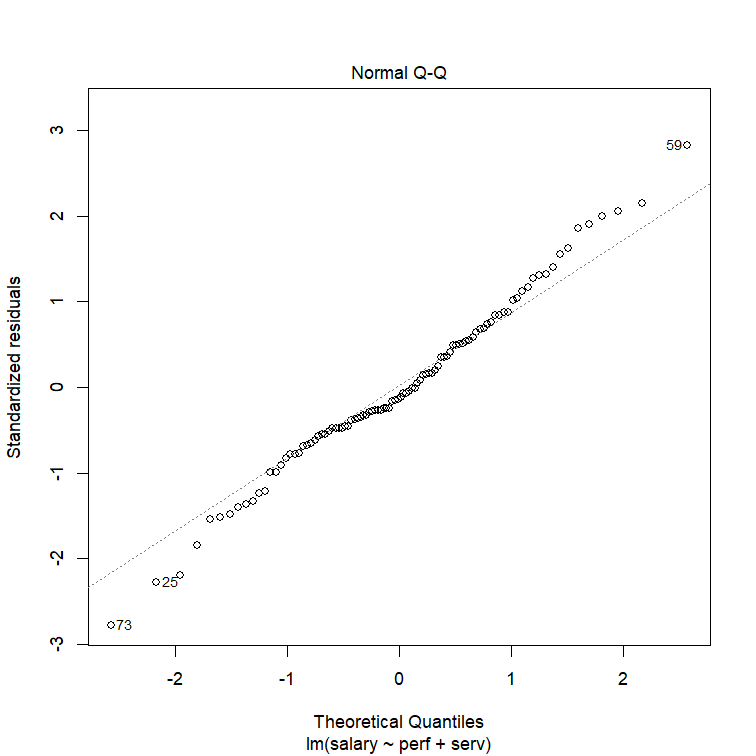
\includegraphics{dapr2_10_CategoricalAnalysisPlan_files/figure-latex/unnamed-chunk-13-1.pdf}

\begin{Shaded}
\begin{Highlighting}[]
\FunctionTok{plot}\NormalTok{(m1, }\AttributeTok{which =} \DecValTok{2}\NormalTok{)}
\end{Highlighting}
\end{Shaded}

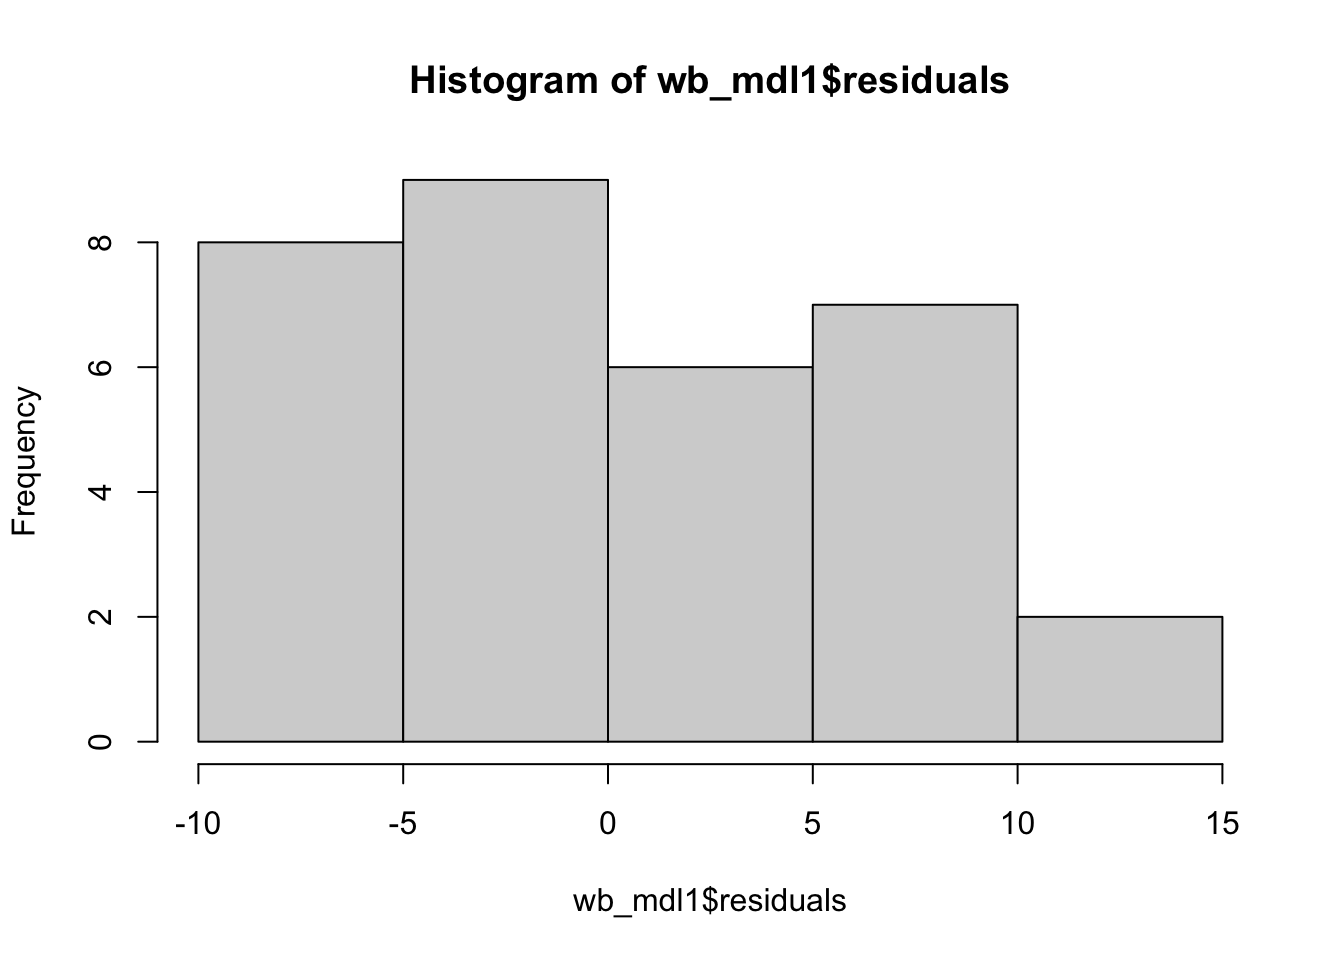
\includegraphics{dapr2_10_CategoricalAnalysisPlan_files/figure-latex/unnamed-chunk-14-1.pdf}

Tails are a bit fatter than we would expect (particularly on the right), but overall, this looks pretty good. No major concerns.

\textbf{Equality of Variance (Homoskedasticity)}
We can check for heteroskedasticity using residuals vs predicted values plots. We can get these using the \texttt{residualPlot} from the \texttt{car} package:

\begin{Shaded}
\begin{Highlighting}[]
\FunctionTok{residualPlot}\NormalTok{(m1)}
\end{Highlighting}
\end{Shaded}

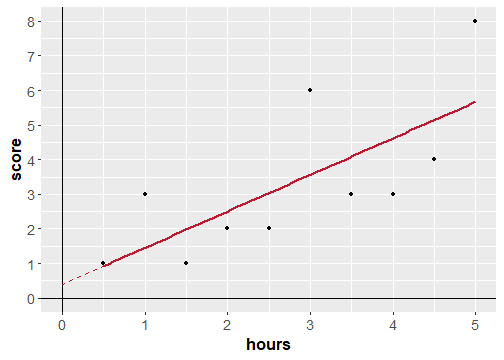
\includegraphics{dapr2_10_CategoricalAnalysisPlan_files/figure-latex/unnamed-chunk-15-1.pdf}

Looks good! Now we can interpret the model.

\begin{Shaded}
\begin{Highlighting}[]
\FunctionTok{summary}\NormalTok{(m1)}
\end{Highlighting}
\end{Shaded}

\begin{verbatim}
## 
## Call:
## lm(formula = Attendance ~ Conscientiousness + OnlineAccess + 
##     Year, data = dat)
## 
## Residuals:
##     Min      1Q  Median      3Q     Max 
## -37.777  -6.996  -0.243   6.079  31.849 
## 
## Coefficients:
##                       Estimate Std. Error t value Pr(>|t|)    
## (Intercept)             27.882      1.533  18.186  < 2e-16 ***
## ConscientiousnessLow   -10.304      1.398  -7.370 1.04e-12 ***
## ConscientiousnessHigh    7.361      1.392   5.288 2.08e-07 ***
## OnlineAccessRarely      -5.387      1.441  -3.738 0.000214 ***
## OnlineAccessOften       -3.535      1.339  -2.640 0.008631 ** 
## YearY2                   4.573      1.657   2.760 0.006064 ** 
## YearY3                   3.534      1.860   1.899 0.058247 .  
## YearY4                   4.150      1.812   2.291 0.022528 *  
## YearMSc                  5.649      2.047   2.760 0.006059 ** 
## YearPhD                 12.483      2.661   4.691 3.78e-06 ***
## ---
## Signif. codes:  0 '***' 0.001 '**' 0.01 '*' 0.05 '.' 0.1 ' ' 1
## 
## Residual standard error: 11.35 on 387 degrees of freedom
## Multiple R-squared:  0.3572, Adjusted R-squared:  0.3423 
## F-statistic:  23.9 on 9 and 387 DF,  p-value: < 2.2e-16
\end{verbatim}

\hypertarget{effects-coding}{%
\paragraph{Effects Coding}\label{effects-coding}}

Now that we've created a model with dummy-coded predictors, let's run the same model with effects coding.

First, let's consider which level we want to drop in each case. Perhaps we're more interested in how the ``extreme'' groups differ from average. We'll drop the \texttt{Moderate} and \texttt{Sometimes} levels from the \texttt{Conscientiousness} and \texttt{OnlineAccess} variables, respectively. We'll drop \texttt{Y3} from our \texttt{Year} variable. To do this, we'll need to reorder our variables accordingly:

\begin{Shaded}
\begin{Highlighting}[]
\NormalTok{dat}\SpecialCharTok{$}\NormalTok{Conscientiousness }\OtherTok{\textless{}{-}}\NormalTok{ dat}\SpecialCharTok{$}\NormalTok{Conscientiousness }\SpecialCharTok{\%\textgreater{}\%} 
  \FunctionTok{factor}\NormalTok{(., }\AttributeTok{levels =} \FunctionTok{c}\NormalTok{(}\StringTok{\textquotesingle{}Low\textquotesingle{}}\NormalTok{, }\StringTok{\textquotesingle{}High\textquotesingle{}}\NormalTok{, }\StringTok{\textquotesingle{}Moderate\textquotesingle{}}\NormalTok{))}

\FunctionTok{summary}\NormalTok{(dat}\SpecialCharTok{$}\NormalTok{Conscientiousness)}
\end{Highlighting}
\end{Shaded}

\begin{verbatim}
##      Low     High Moderate 
##      127      124      146
\end{verbatim}

\begin{Shaded}
\begin{Highlighting}[]
\NormalTok{dat}\SpecialCharTok{$}\NormalTok{OnlineAccess }\OtherTok{\textless{}{-}}\NormalTok{ dat}\SpecialCharTok{$}\NormalTok{OnlineAccess }\SpecialCharTok{\%\textgreater{}\%} 
  \FunctionTok{factor}\NormalTok{(., }\AttributeTok{levels =} \FunctionTok{c}\NormalTok{(}\StringTok{\textquotesingle{}Rarely\textquotesingle{}}\NormalTok{, }\StringTok{\textquotesingle{}Often\textquotesingle{}}\NormalTok{, }\StringTok{\textquotesingle{}Sometimes\textquotesingle{}}\NormalTok{))}

\FunctionTok{summary}\NormalTok{(dat}\SpecialCharTok{$}\NormalTok{OnlineAccess)}
\end{Highlighting}
\end{Shaded}

\begin{verbatim}
##    Rarely     Often Sometimes 
##       101       126       170
\end{verbatim}

\begin{Shaded}
\begin{Highlighting}[]
\NormalTok{dat}\SpecialCharTok{$}\NormalTok{Year }\OtherTok{\textless{}{-}}\NormalTok{ dat}\SpecialCharTok{$}\NormalTok{Year }\SpecialCharTok{\%\textgreater{}\%} 
  \FunctionTok{factor}\NormalTok{(., }\AttributeTok{levels =} \FunctionTok{c}\NormalTok{(}\StringTok{\textquotesingle{}Y1\textquotesingle{}}\NormalTok{, }\StringTok{\textquotesingle{}Y2\textquotesingle{}}\NormalTok{, }\StringTok{\textquotesingle{}Y4\textquotesingle{}}\NormalTok{, }\StringTok{\textquotesingle{}MSc\textquotesingle{}}\NormalTok{, }\StringTok{\textquotesingle{}PhD\textquotesingle{}}\NormalTok{, }\StringTok{\textquotesingle{}Y3\textquotesingle{}}\NormalTok{))}

\FunctionTok{summary}\NormalTok{(dat}\SpecialCharTok{$}\NormalTok{Year)}
\end{Highlighting}
\end{Shaded}

\begin{verbatim}
##  Y1  Y2  Y4 MSc PhD  Y3 
##  89 100  72  48  23  65
\end{verbatim}

We also need to specify effects coding using the \texttt{contr.sum} function:

\begin{Shaded}
\begin{Highlighting}[]
\FunctionTok{contrasts}\NormalTok{(dat}\SpecialCharTok{$}\NormalTok{Conscientiousness) }\OtherTok{\textless{}{-}}\NormalTok{ contr.sum}
\FunctionTok{contrasts}\NormalTok{(dat}\SpecialCharTok{$}\NormalTok{OnlineAccess) }\OtherTok{\textless{}{-}}\NormalTok{ contr.sum}
\FunctionTok{contrasts}\NormalTok{(dat}\SpecialCharTok{$}\NormalTok{Year) }\OtherTok{\textless{}{-}}\NormalTok{ contr.sum}
\end{Highlighting}
\end{Shaded}

Now we can run our model. Keep in mind that we don't need to recheck assumptions. The data are the same, it's just the comparisons that differ.

\begin{Shaded}
\begin{Highlighting}[]
\NormalTok{m2 }\OtherTok{\textless{}{-}} \FunctionTok{lm}\NormalTok{(Attendance}\SpecialCharTok{\textasciitilde{}}\NormalTok{Conscientiousness}\SpecialCharTok{+}\NormalTok{OnlineAccess}\SpecialCharTok{+}\NormalTok{Year, dat)}
\FunctionTok{summary}\NormalTok{(m2)}
\end{Highlighting}
\end{Shaded}

\begin{verbatim}
## 
## Call:
## lm(formula = Attendance ~ Conscientiousness + OnlineAccess + 
##     Year, data = dat)
## 
## Residuals:
##     Min      1Q  Median      3Q     Max 
## -37.777  -6.996  -0.243   6.079  31.849 
## 
## Coefficients:
##                    Estimate Std. Error t value Pr(>|t|)    
## (Intercept)         28.9921     0.6545  44.296  < 2e-16 ***
## Conscientiousness1  -9.3232     0.8278 -11.262  < 2e-16 ***
## Conscientiousness2   8.3421     0.8244  10.119  < 2e-16 ***
## OnlineAccess1       -2.4128     0.8850  -2.727 0.006692 ** 
## OnlineAccess2       -0.5609     0.8298  -0.676 0.499436    
## Year1               -5.0648     1.1784  -4.298 2.18e-05 ***
## Year2               -0.4914     1.1293  -0.435 0.663726    
## Year3               -0.9146     1.2725  -0.719 0.472740    
## Year4                0.5838     1.4890   0.392 0.695223    
## Year5                7.4179     2.0436   3.630 0.000322 ***
## ---
## Signif. codes:  0 '***' 0.001 '**' 0.01 '*' 0.05 '.' 0.1 ' ' 1
## 
## Residual standard error: 11.35 on 387 degrees of freedom
## Multiple R-squared:  0.3572, Adjusted R-squared:  0.3423 
## F-statistic:  23.9 on 9 and 387 DF,  p-value: < 2.2e-16
\end{verbatim}

This isn't entirely necessary, but here I'm just going to create some objects to use for inline coding in the example.

\begin{Shaded}
\begin{Highlighting}[]
\NormalTok{sumM2 }\OtherTok{\textless{}{-}} \FunctionTok{summary}\NormalTok{(m2)}
\NormalTok{FDat }\OtherTok{\textless{}{-}} \FunctionTok{round}\NormalTok{(sumM2}\SpecialCharTok{$}\NormalTok{fstatistic, }\DecValTok{2}\NormalTok{)}
\NormalTok{m2Coefs }\OtherTok{\textless{}{-}} \FunctionTok{round}\NormalTok{(}\FunctionTok{coef}\NormalTok{(m2), }\DecValTok{2}\NormalTok{)}
\NormalTok{tStats }\OtherTok{\textless{}{-}} \FunctionTok{round}\NormalTok{(}\FunctionTok{coef}\NormalTok{(sumM2)[, }\StringTok{"t value"}\NormalTok{],}\DecValTok{2}\NormalTok{)}
\NormalTok{seVals }\OtherTok{\textless{}{-}} \FunctionTok{round}\NormalTok{(}\FunctionTok{coef}\NormalTok{(sumM2)[, }\StringTok{"Std. Error"}\NormalTok{],}\DecValTok{2}\NormalTok{)}
\end{Highlighting}
\end{Shaded}

\hypertarget{sample-write-up-and-model-interpretation-rq1--}{%
\subsubsection{Sample write up and model interpretation, RQ1 -}\label{sample-write-up-and-model-interpretation-rq1--}}

We will be evaluating all results using \(\alpha = .05\).

Looking at these results, we can see that our overall model is significant, \(F(9, 387) = 23.9, p < .001\). Conscientiousness, frequency of online access, and year in university explain 34\% of the variance in attendance. Both those with high and low levels of conscientiousness exhibited attendance rates that were significantly different than average (See Figure \ref{fig:conscFig}). Specifically, those with high levels of conscientiousness attended class significantly more often than average, \(\beta = 8.34, SE = 0.82, t = 10.12, p < .001\). Conversely, those with low levels of conscientiousness attended class significantly less than average, \(\beta = -9.32, SE = 0.83, t = -11.26, p < .001\). Specifically, those with low levels of conscientiousness attended, on average, -9.32 fewer class periods than average, when controlling for year of study and online access.

\begin{Shaded}
\begin{Highlighting}[]
\NormalTok{dat }\SpecialCharTok{\%\textgreater{}\%}
  \FunctionTok{filter}\NormalTok{(Conscientiousness }\SpecialCharTok{!=} \StringTok{\textquotesingle{}Moderate\textquotesingle{}}\NormalTok{) }\SpecialCharTok{\%\textgreater{}\%}
  \FunctionTok{ggplot}\NormalTok{(., }\FunctionTok{aes}\NormalTok{(Conscientiousness, Attendance, }\AttributeTok{colour =}\NormalTok{ Conscientiousness)) }\SpecialCharTok{+} 
  \FunctionTok{geom\_boxplot}\NormalTok{(}\AttributeTok{width =}\NormalTok{ .}\DecValTok{5}\NormalTok{) }\SpecialCharTok{+} 
  \FunctionTok{geom\_jitter}\NormalTok{(}\AttributeTok{width =}\NormalTok{ .}\DecValTok{2}\NormalTok{, }\AttributeTok{alpha =}\NormalTok{ .}\DecValTok{5}\NormalTok{) }\SpecialCharTok{+} 
  \FunctionTok{theme}\NormalTok{(}\AttributeTok{legend.position =} \StringTok{\textquotesingle{}none\textquotesingle{}}\NormalTok{,}
        \AttributeTok{axis.title =} \FunctionTok{element\_text}\NormalTok{(}\AttributeTok{size =} \DecValTok{14}\NormalTok{, }\AttributeTok{face =} \StringTok{\textquotesingle{}bold\textquotesingle{}}\NormalTok{),}
        \AttributeTok{axis.text =} \FunctionTok{element\_text}\NormalTok{(}\AttributeTok{size =} \DecValTok{12}\NormalTok{))}
\end{Highlighting}
\end{Shaded}

\begin{figure}
\centering
\includegraphics{dapr2_10_CategoricalAnalysisPlan_files/figure-latex/conscFig-1.pdf}
\caption{\label{fig:conscFig}Attendance by Level of Conscientiousness}
\end{figure}

Both those who often accessed the online materials (REPORT BETA, SE, T, and P HERE) and those who rarely accessed the online materials (REPORT BETA, SE, T, and P HERE) attended class less often than those who sometimes accessed the online content (See FIG 3).
Students in Y1 attended approximately BETA fewer courses than the average student (REPORT BETA, SE, T, and P HERE), while PhD students attended approximately BETA more courses than the average student (REPORT BETA, SE, T, and P HERE). There was no signifiant difference in the average number of courses attended by the other year groups. Please see Table X for descriptive data on attendance by group.

NOTE FOR EMMA:
Will make plots for each of the predictors. This is just the base example of what I plan to do for each:

\begin{Shaded}
\begin{Highlighting}[]
\FunctionTok{ggplot}\NormalTok{(dat, }\FunctionTok{aes}\NormalTok{(OnlineAccess, Attendance, }\AttributeTok{colour =}\NormalTok{ OnlineAccess)) }\SpecialCharTok{+} \FunctionTok{geom\_boxplot}\NormalTok{() }\SpecialCharTok{+} \FunctionTok{geom\_jitter}\NormalTok{(}\FunctionTok{aes}\NormalTok{(}\AttributeTok{color =}\NormalTok{ OnlineAccess)) }\SpecialCharTok{+}
  \FunctionTok{theme}\NormalTok{(}\AttributeTok{legend.position =} \StringTok{\textquotesingle{}none\textquotesingle{}}\NormalTok{)}
\end{Highlighting}
\end{Shaded}

\begin{figure}
\centering
\includegraphics{dapr2_10_CategoricalAnalysisPlan_files/figure-latex/fig3-1.pdf}
\caption{\label{fig:fig3}Student Attendance by Online Material Access}
\end{figure}

TABLE HERE WITH MEAN AND SD of ATTENDANCE BY EACH GROUP.

\hypertarget{aim-2---contrast-coding-change-this-heading}{%
\subsection{Aim 2 - Contrast Coding (CHANGE THIS HEADING)}\label{aim-2---contrast-coding-change-this-heading}}

Our second research question is \textbf{Is the time at which the class is scheduled associated with student attendance?}. To test this, we'll use the \texttt{emmeans} function to write our own contrasts. We're going to be testing the following model:

\[Attendance \sim Time\]

First, let's relevel our \texttt{Time\ variable} so that it's in chronological order:

\begin{Shaded}
\begin{Highlighting}[]
\NormalTok{dat}\SpecialCharTok{$}\NormalTok{Time }\OtherTok{\textless{}{-}}\NormalTok{ dat}\SpecialCharTok{$}\NormalTok{Time }\SpecialCharTok{\%\textgreater{}\%} 
  \FunctionTok{factor}\NormalTok{(., }\AttributeTok{levels =} \FunctionTok{c}\NormalTok{(}\StringTok{\textquotesingle{}9AM\textquotesingle{}}\NormalTok{, }\StringTok{\textquotesingle{}10AM\textquotesingle{}}\NormalTok{, }\StringTok{\textquotesingle{}11AM\textquotesingle{}}\NormalTok{,}\StringTok{\textquotesingle{}12PM\textquotesingle{}}\NormalTok{, }\StringTok{\textquotesingle{}1PM\textquotesingle{}}\NormalTok{, }\StringTok{\textquotesingle{}2PM\textquotesingle{}}\NormalTok{, }\StringTok{\textquotesingle{}3PM\textquotesingle{}}\NormalTok{, }\StringTok{\textquotesingle{}4PM\textquotesingle{}}\NormalTok{))}

\FunctionTok{summary}\NormalTok{(dat}\SpecialCharTok{$}\NormalTok{Time)}
\end{Highlighting}
\end{Shaded}

\begin{verbatim}
##  9AM 10AM 11AM 12PM  1PM  2PM  3PM  4PM 
##   56   48   46   47   45   46   52   57
\end{verbatim}

We'll look at how \texttt{Time} is distributed using a bar plot:

\begin{Shaded}
\begin{Highlighting}[]
\FunctionTok{ggplot}\NormalTok{(dat, }\FunctionTok{aes}\NormalTok{(Time, }\AttributeTok{fill =}\NormalTok{ Time)) }\SpecialCharTok{+} \FunctionTok{geom\_bar}\NormalTok{() }\SpecialCharTok{+} 
  \FunctionTok{theme}\NormalTok{(}\AttributeTok{legend.position =} \StringTok{\textquotesingle{}none\textquotesingle{}}\NormalTok{)}
\end{Highlighting}
\end{Shaded}

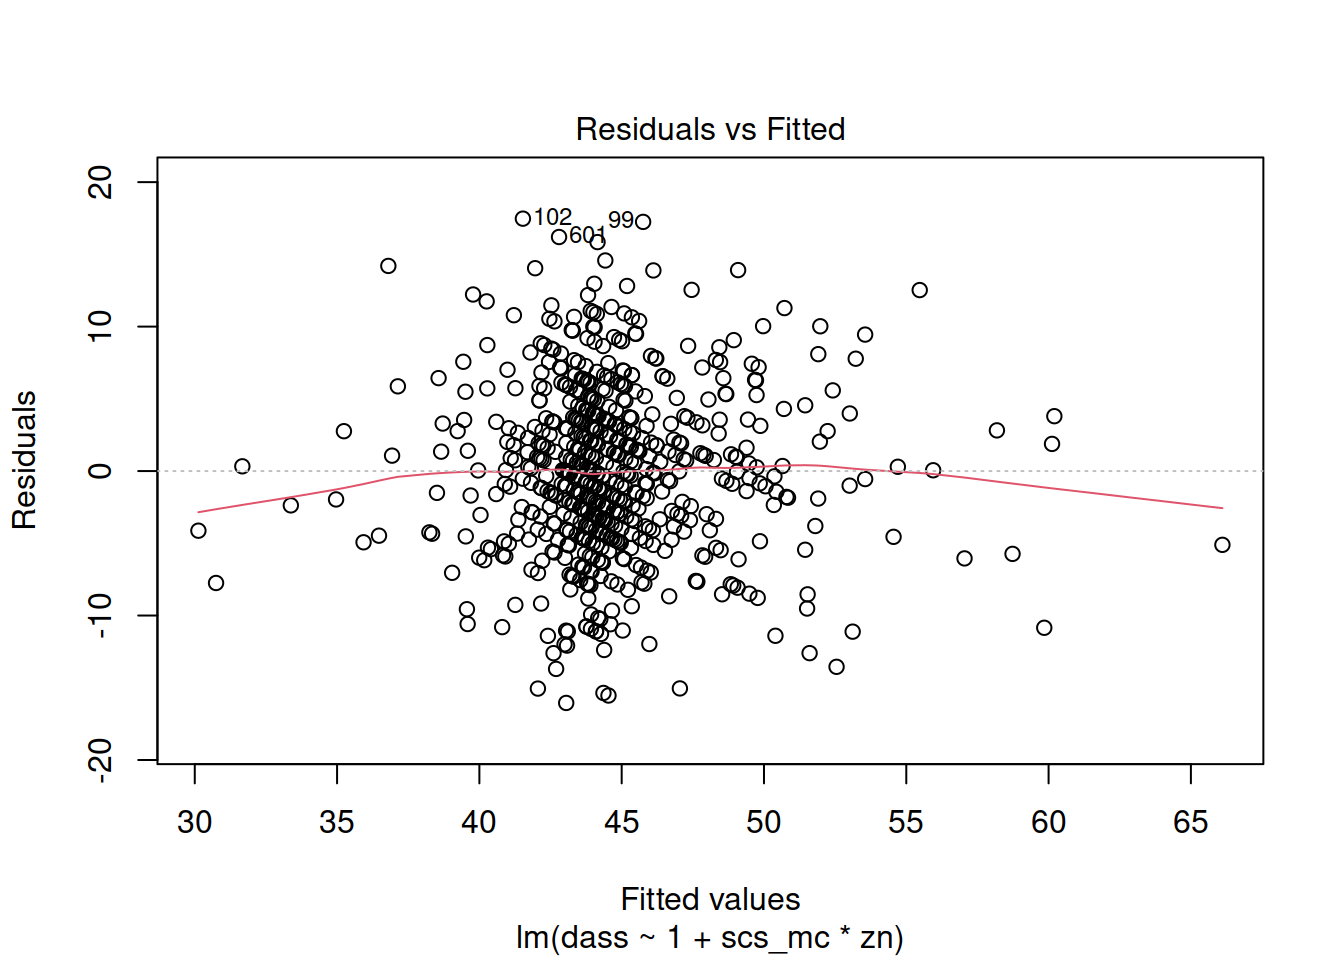
\includegraphics{dapr2_10_CategoricalAnalysisPlan_files/figure-latex/unnamed-chunk-24-1.pdf}
First let's run our model and check assumptions. Remember, we don't need to check linearity or independence.

\textbf{Normality of residuals:}

\begin{Shaded}
\begin{Highlighting}[]
\NormalTok{m3 }\OtherTok{\textless{}{-}} \FunctionTok{lm}\NormalTok{(Attendance}\SpecialCharTok{\textasciitilde{}}\NormalTok{Time, dat)}

\FunctionTok{hist}\NormalTok{(m3}\SpecialCharTok{$}\NormalTok{residuals)}
\end{Highlighting}
\end{Shaded}

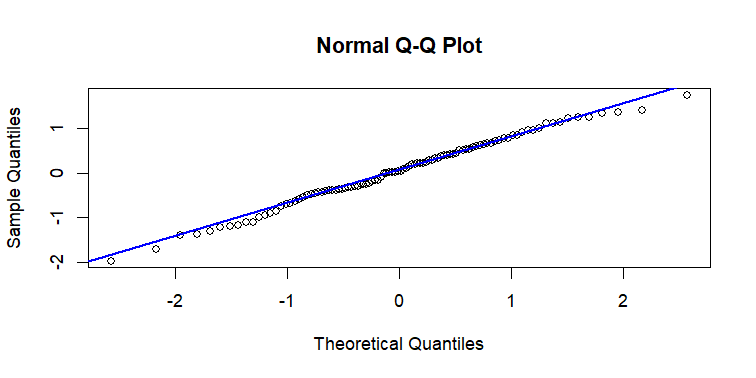
\includegraphics{dapr2_10_CategoricalAnalysisPlan_files/figure-latex/unnamed-chunk-25-1.pdf}

\begin{Shaded}
\begin{Highlighting}[]
\FunctionTok{plot}\NormalTok{(m3, }\AttributeTok{which =} \DecValTok{2}\NormalTok{)}
\end{Highlighting}
\end{Shaded}

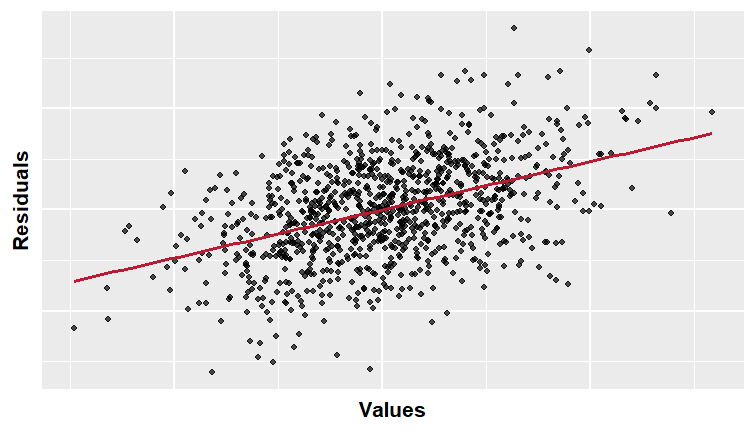
\includegraphics{dapr2_10_CategoricalAnalysisPlan_files/figure-latex/unnamed-chunk-26-1.pdf}
The distribution is a bit flat, but if you'll remember from class, distributional problems are usually not a strong concern (and we can always bootstrap for extra certainty!). Heteroskedasticity is much more of a problem. Let's check that using our residual by predicted values plot.

\begin{Shaded}
\begin{Highlighting}[]
\FunctionTok{residualPlot}\NormalTok{(m3)}
\end{Highlighting}
\end{Shaded}

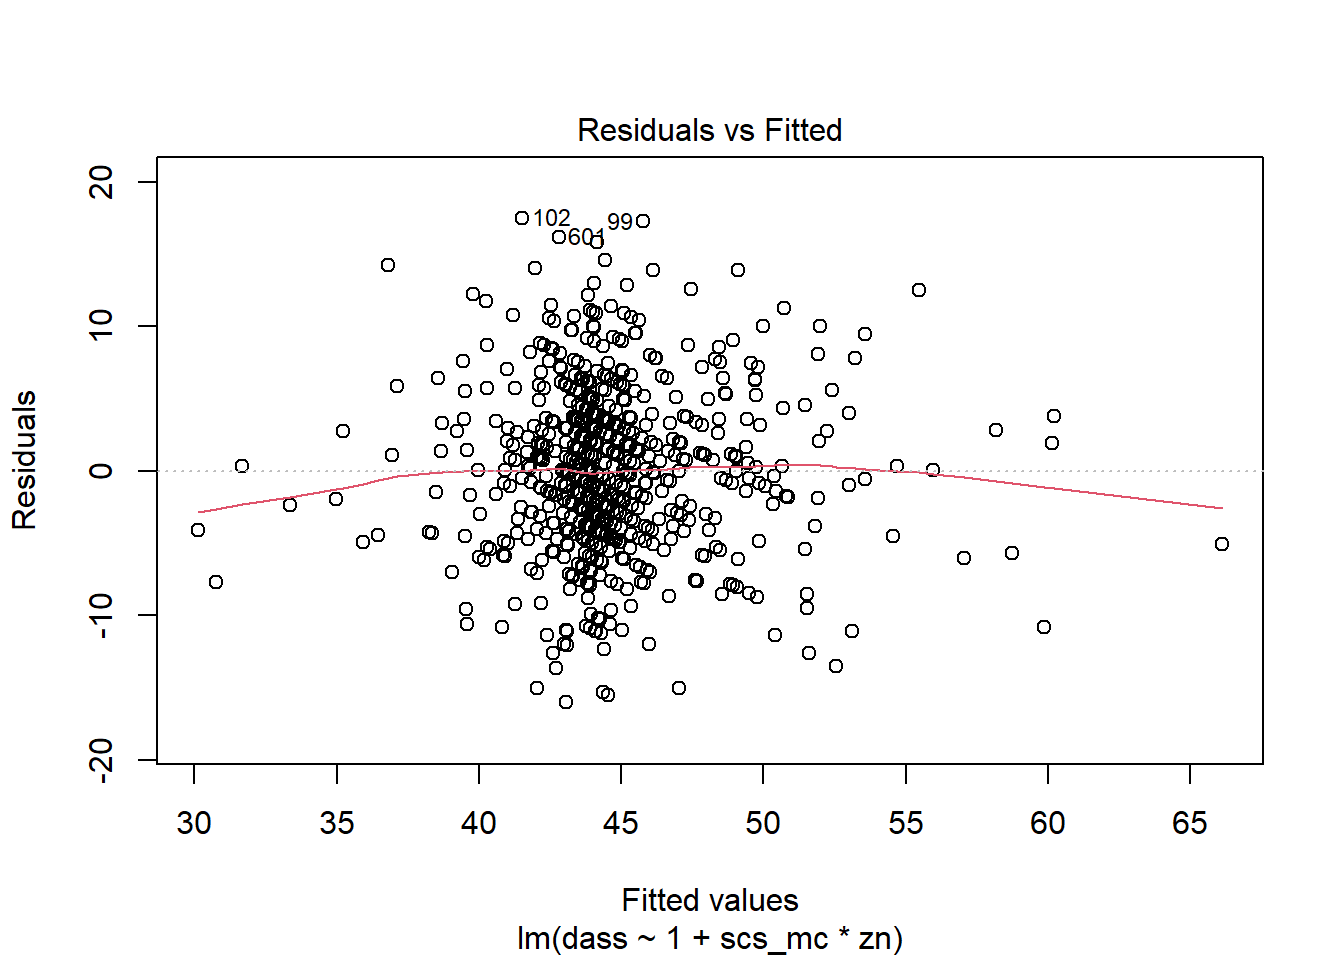
\includegraphics{dapr2_10_CategoricalAnalysisPlan_files/figure-latex/unnamed-chunk-27-1.pdf}

This looks great! We're going to keep our model as is.

Now let's specify our contrasts with emmeans:

\begin{Shaded}
\begin{Highlighting}[]
\NormalTok{(timeMean }\OtherTok{\textless{}{-}} \FunctionTok{emmeans}\NormalTok{(m3, }\SpecialCharTok{\textasciitilde{}}\NormalTok{Time))}
\end{Highlighting}
\end{Shaded}

\begin{verbatim}
##  Time emmean   SE  df lower.CL upper.CL
##  9AM    20.1 1.79 389     16.6     23.6
##  10AM   27.0 1.94 389     23.2     30.8
##  11AM   27.8 1.98 389     23.9     31.7
##  12PM   31.3 1.96 389     27.5     35.1
##  1PM    33.5 2.00 389     29.5     37.4
##  2PM    32.4 1.98 389     28.5     36.3
##  3PM    31.7 1.86 389     28.0     35.3
##  4PM    24.8 1.78 389     21.3     28.2
## 
## Confidence level used: 0.95
\end{verbatim}

\begin{Shaded}
\begin{Highlighting}[]
\FunctionTok{plot}\NormalTok{(timeMean)}
\end{Highlighting}
\end{Shaded}

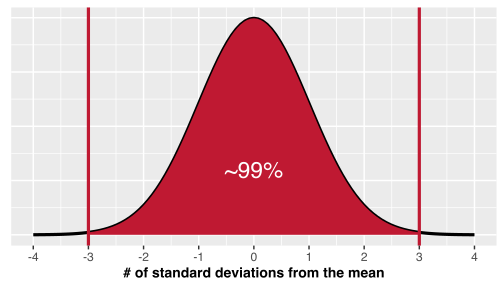
\includegraphics{dapr2_10_CategoricalAnalysisPlan_files/figure-latex/unnamed-chunk-29-1.pdf}

I'd guess we're going to see some significant differences here. Let's say, however, we're less worried about specific times and more about times of day in general.

\begin{Shaded}
\begin{Highlighting}[]
\FunctionTok{levels}\NormalTok{(dat}\SpecialCharTok{$}\NormalTok{Time)}
\end{Highlighting}
\end{Shaded}

\begin{verbatim}
## [1] "9AM"  "10AM" "11AM" "12PM" "1PM"  "2PM"  "3PM"  "4PM"
\end{verbatim}

\begin{Shaded}
\begin{Highlighting}[]
\NormalTok{timeComp }\OtherTok{\textless{}{-}} \FunctionTok{list}\NormalTok{(}\StringTok{\textquotesingle{}Early or Late vs Middle of the Day\textquotesingle{}} \OtherTok{=} \FunctionTok{c}\NormalTok{(}\SpecialCharTok{{-}}\DecValTok{1}\SpecialCharTok{/}\DecValTok{4}\NormalTok{,}\SpecialCharTok{{-}}\DecValTok{1}\SpecialCharTok{/}\DecValTok{4}\NormalTok{, }\DecValTok{1}\SpecialCharTok{/}\DecValTok{4}\NormalTok{, }\DecValTok{1}\SpecialCharTok{/}\DecValTok{4}\NormalTok{, }\DecValTok{1}\SpecialCharTok{/}\DecValTok{4}\NormalTok{, }\DecValTok{1}\SpecialCharTok{/}\DecValTok{4}\NormalTok{, }\SpecialCharTok{{-}}\DecValTok{1}\SpecialCharTok{/}\DecValTok{4}\NormalTok{, }\SpecialCharTok{{-}}\DecValTok{1}\SpecialCharTok{/}\DecValTok{4}\NormalTok{))}
\end{Highlighting}
\end{Shaded}

\begin{Shaded}
\begin{Highlighting}[]
\NormalTok{(timeTest }\OtherTok{\textless{}{-}} \FunctionTok{contrast}\NormalTok{(timeMean, timeComp))}
\end{Highlighting}
\end{Shaded}

\begin{verbatim}
##  contrast                           estimate   SE  df t.ratio p.value
##  Early or Late vs Middle of the Day     5.36 1.35 389   3.963  0.0001
\end{verbatim}

Here, we see that students with classes in the middle of the day are more likely to attend than those who have classes either early in the morning or later in the afternoon (REPORT NUMERIC RESULTS HERE).

\hypertarget{study-2}{%
\section{Study 2}\label{study-2}}

We collected attendance and final mark data from 200 university students.

\begin{longtable}{ll}
\toprule
Variable & Description \\ 
\midrule
Marks & Total attendance in days \\ 
Attendance & Final Mark in points \\ 
\bottomrule
\end{longtable}

We want to use these data to investigate the following research question:

\textbf{Research Question:} Can student attendance be used to predict marks?

\hypertarget{study-2-setup}{%
\subsection{Study 2 Setup}\label{study-2-setup}}

First, let's load the data.

\begin{Shaded}
\begin{Highlighting}[]
\NormalTok{dat2 }\OtherTok{\textless{}{-}} \FunctionTok{read.csv}\NormalTok{(}\StringTok{\textquotesingle{}https://uoepsy.github.io/data/DapR2\_S1B2\_PracticalPart2.csv\textquotesingle{}}\NormalTok{, }\AttributeTok{stringsAsFactors =}\NormalTok{ T)}
\end{Highlighting}
\end{Shaded}

\hypertarget{study-2---checking-the-data}{%
\subsection{Study 2 - Checking the Data}\label{study-2---checking-the-data}}

First, let's have a look at the data:

\begin{Shaded}
\begin{Highlighting}[]
\NormalTok{dat2 }\SpecialCharTok{\%\textgreater{}\%}
  \FunctionTok{summary}\NormalTok{(.)}
\end{Highlighting}
\end{Shaded}

\begin{verbatim}
##      Marks         Attendance   
##  Min.   :25.01   Min.   :10.50  
##  1st Qu.:38.22   1st Qu.:22.88  
##  Median :48.81   Median :35.25  
##  Mean   :49.79   Mean   :35.25  
##  3rd Qu.:60.90   3rd Qu.:47.62  
##  Max.   :98.20   Max.   :60.00
\end{verbatim}

You'll notice that here we have two continuous outcome variables, \texttt{Attendance} and \texttt{Marks}.

Let's look at how our variables are distributed, using histograms:

\begin{Shaded}
\begin{Highlighting}[]
\FunctionTok{ggplot}\NormalTok{(dat2, }\FunctionTok{aes}\NormalTok{(Attendance)) }\SpecialCharTok{+} \FunctionTok{geom\_histogram}\NormalTok{(}\AttributeTok{colour =} \StringTok{\textquotesingle{}black\textquotesingle{}}\NormalTok{)}
\end{Highlighting}
\end{Shaded}

\begin{verbatim}
## `stat_bin()` using `bins = 30`. Pick better value with `binwidth`.
\end{verbatim}

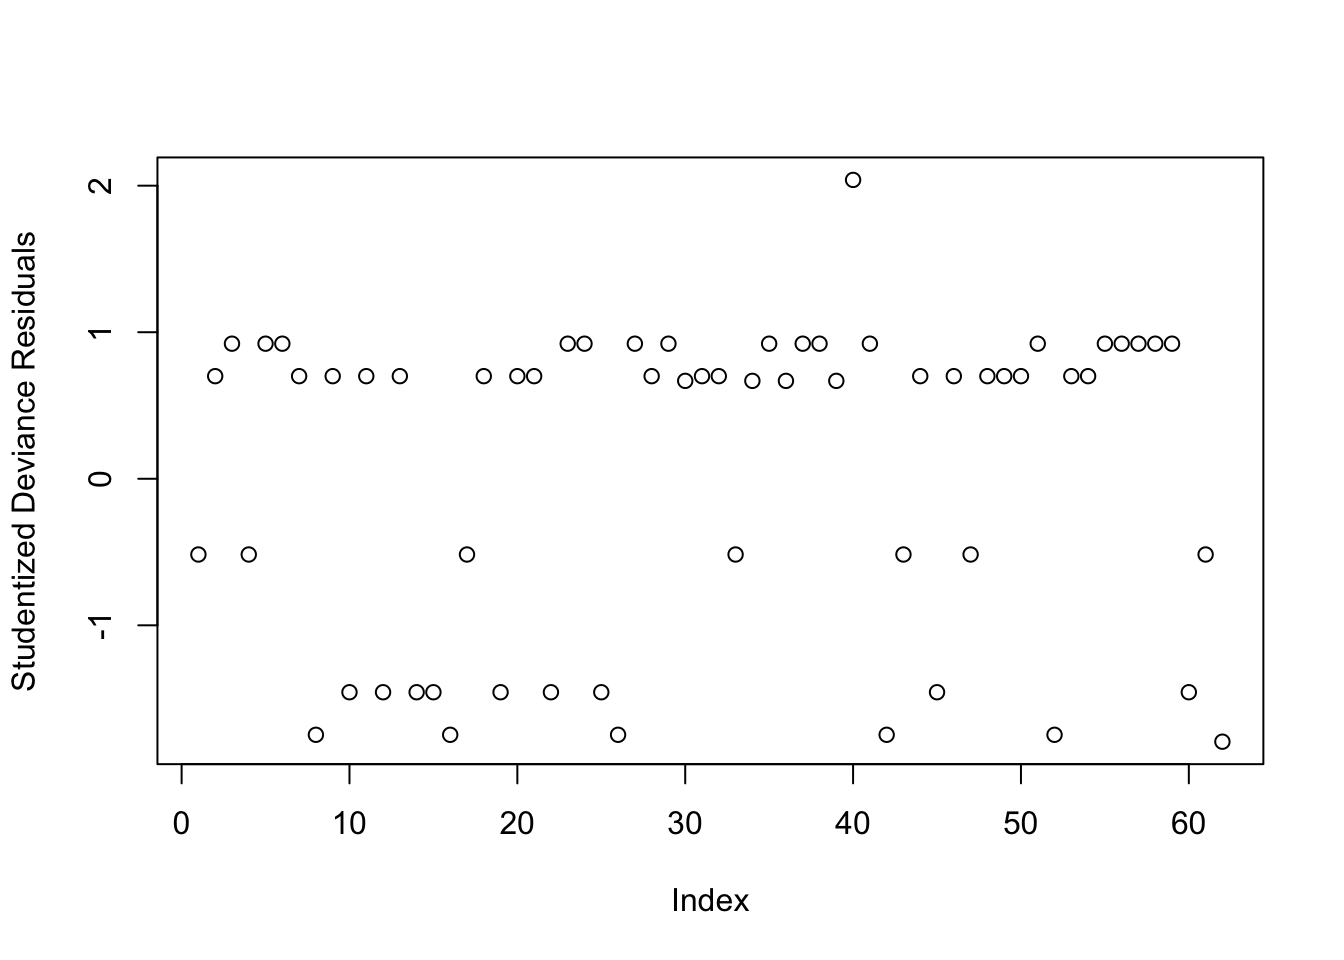
\includegraphics{dapr2_10_CategoricalAnalysisPlan_files/figure-latex/unnamed-chunk-35-1.pdf}
Ok, that looks a bit weird\ldots but let's keep going.

\begin{Shaded}
\begin{Highlighting}[]
\FunctionTok{ggplot}\NormalTok{(dat2, }\FunctionTok{aes}\NormalTok{(Marks)) }\SpecialCharTok{+} \FunctionTok{geom\_histogram}\NormalTok{(}\AttributeTok{colour =} \StringTok{\textquotesingle{}black\textquotesingle{}}\NormalTok{, }\AttributeTok{binwidth =} \DecValTok{4}\NormalTok{)}
\end{Highlighting}
\end{Shaded}

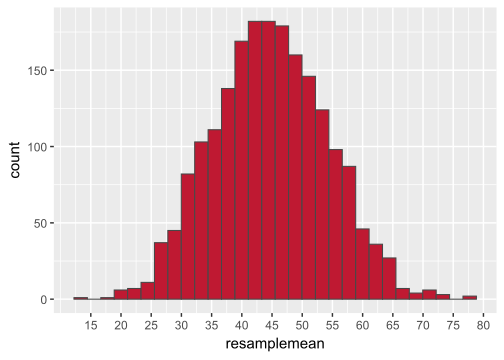
\includegraphics{dapr2_10_CategoricalAnalysisPlan_files/figure-latex/unnamed-chunk-36-1.pdf}

\hypertarget{study-2---modelling-change-this-heading}{%
\section{Study 2 - Modelling (CHANGE THIS HEADING)}\label{study-2---modelling-change-this-heading}}

We'll use the following model to investigate our research question:

\[Attendance \sim Time\]

Let's run our model, then we'll check assumptions:

\begin{Shaded}
\begin{Highlighting}[]
\NormalTok{m4 }\OtherTok{\textless{}{-}} \FunctionTok{lm}\NormalTok{(Marks}\SpecialCharTok{\textasciitilde{}}\NormalTok{Attendance, dat2)}
\FunctionTok{summary}\NormalTok{(m4)}
\end{Highlighting}
\end{Shaded}

\begin{verbatim}
## 
## Call:
## lm(formula = Marks ~ Attendance, data = dat2)
## 
## Residuals:
##      Min       1Q   Median       3Q      Max 
## -17.1477  -4.5210  -0.1861   4.2501  26.8415 
## 
## Coefficients:
##             Estimate Std. Error t value Pr(>|t|)    
## (Intercept) 14.83270    1.25534   11.82   <2e-16 ***
## Attendance   0.99163    0.03296   30.09   <2e-16 ***
## ---
## Signif. codes:  0 '***' 0.001 '**' 0.01 '*' 0.05 '.' 0.1 ' ' 1
## 
## Residual standard error: 6.727 on 198 degrees of freedom
## Multiple R-squared:  0.8205, Adjusted R-squared:  0.8196 
## F-statistic: 905.3 on 1 and 198 DF,  p-value: < 2.2e-16
\end{verbatim}

This model looks highly significant, but we'll have to check assumptions before interpretation, especially given how the distribution of attendance looked.

\textbf{Linearity}
It's a simple regression, so we can just look at the scatterplot:

\begin{Shaded}
\begin{Highlighting}[]
\FunctionTok{ggplot}\NormalTok{(dat2, }\FunctionTok{aes}\NormalTok{(Attendance, Marks)) }\SpecialCharTok{+} \FunctionTok{geom\_point}\NormalTok{() }\SpecialCharTok{+} 
  \FunctionTok{geom\_smooth}\NormalTok{(}\AttributeTok{method =} \StringTok{\textquotesingle{}lm\textquotesingle{}}\NormalTok{) }\SpecialCharTok{+} 
  \FunctionTok{geom\_smooth}\NormalTok{(}\AttributeTok{method =} \StringTok{\textquotesingle{}loess\textquotesingle{}}\NormalTok{, }\AttributeTok{colour =} \StringTok{\textquotesingle{}red\textquotesingle{}}\NormalTok{)}
\end{Highlighting}
\end{Shaded}

\begin{verbatim}
## `geom_smooth()` using formula = 'y ~ x'
## `geom_smooth()` using formula = 'y ~ x'
\end{verbatim}

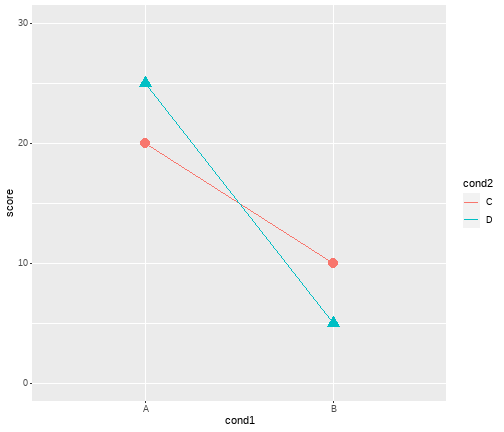
\includegraphics{dapr2_10_CategoricalAnalysisPlan_files/figure-latex/unnamed-chunk-38-1.pdf}

There's a very slight curve in the loess line, but based on the points, I think that's due to possible issues in the distribution of the observations rather than a nonlinear relationship. We'll say linearity assumption is not violated.

\textbf{Independence of Errors}
We are using between-subjects data, so we'll assume independence of our error terms.

\textbf{Normality of Residuals}
Let's check with a histogram and QQ plot:

\begin{Shaded}
\begin{Highlighting}[]
\FunctionTok{hist}\NormalTok{(m4}\SpecialCharTok{$}\NormalTok{residuals)}
\end{Highlighting}
\end{Shaded}

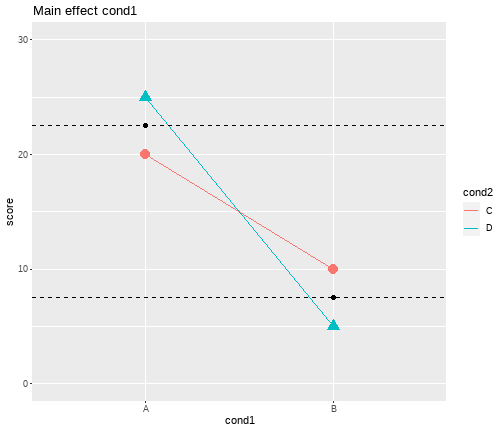
\includegraphics{dapr2_10_CategoricalAnalysisPlan_files/figure-latex/unnamed-chunk-39-1.pdf}
Bit of a tail to the right, but not bad\ldots{}

\begin{Shaded}
\begin{Highlighting}[]
\FunctionTok{plot}\NormalTok{(m4, }\AttributeTok{which =} \DecValTok{2}\NormalTok{)}
\end{Highlighting}
\end{Shaded}

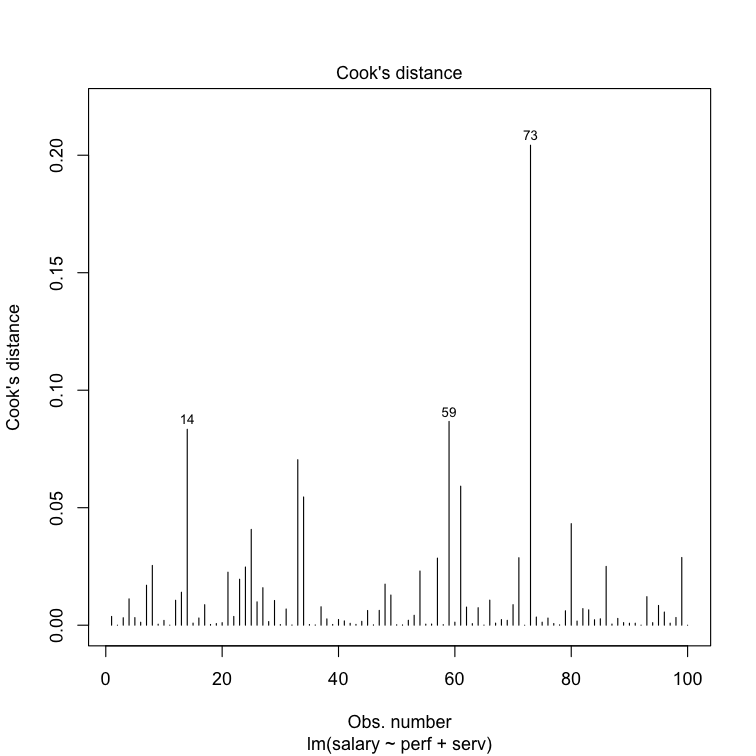
\includegraphics{dapr2_10_CategoricalAnalysisPlan_files/figure-latex/unnamed-chunk-40-1.pdf}
Ok, this actually looks alright, I think. Just the slight tail to the right.

\textbf{Equality of Variance (Homoskedasticity)}
We'll use the \texttt{residualPlot} to check for heteroskedasticity:

\begin{Shaded}
\begin{Highlighting}[]
\FunctionTok{residualPlot}\NormalTok{(m4)}
\end{Highlighting}
\end{Shaded}

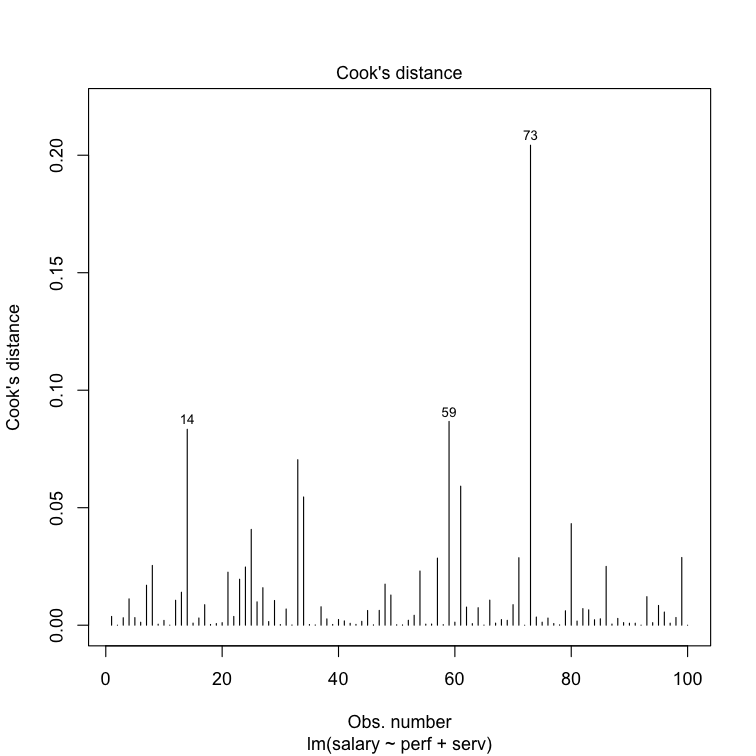
\includegraphics{dapr2_10_CategoricalAnalysisPlan_files/figure-latex/unnamed-chunk-41-1.pdf}
Oh no! It's violated! We can't trust the SEs in our model! We'll need to bootstrap. We can do this using the \texttt{Boot} function in the \texttt{car} package. Let's resample 1000 times.

\begin{Shaded}
\begin{Highlighting}[]
\NormalTok{boot\_m4 }\OtherTok{\textless{}{-}} \FunctionTok{Boot}\NormalTok{(m4, }\AttributeTok{R =} \DecValTok{1000}\NormalTok{)}
\end{Highlighting}
\end{Shaded}

\begin{verbatim}
## Loading required namespace: boot
\end{verbatim}

\begin{Shaded}
\begin{Highlighting}[]
\FunctionTok{summary}\NormalTok{(boot\_m4)}
\end{Highlighting}
\end{Shaded}

\begin{verbatim}
## 
## Number of bootstrap replications R = 1000 
##             original    bootBias   bootSE  bootMed
## (Intercept) 14.83270 -0.01508172 1.033596 14.83955
## Attendance   0.99163  0.00044974 0.036132  0.99086
\end{verbatim}

Let's calculate confidence intervals to test our hypothesis:

\begin{Shaded}
\begin{Highlighting}[]
\FunctionTok{confint}\NormalTok{(boot\_m4)}
\end{Highlighting}
\end{Shaded}

\begin{verbatim}
## Bootstrap bca confidence intervals
## 
##                  2.5 %    97.5 %
## (Intercept) 12.6603636 16.777484
## Attendance   0.9247583  1.068449
\end{verbatim}

Because our confidence interval for the beta associated with attendance does not include 0, we can be more certain that attendance is, in fact, a significant predictor of marks.

WRITE UP HERE\ldots I'M GOING TO BASE THIS ON THE BOOTSTRAP WRITE UP IN THE BOOSTRAPPING LAB.

\end{document}
